\documentclass[conference]{IEEEtran}

\IEEEoverridecommandlockouts
% The preceding line is only needed to identify funding in the first footnote. If that is unneeded, please comment it out.
\usepackage{cite}
\usepackage{amsmath,amssymb,amsfonts}
\usepackage{algorithmic}
\usepackage{graphicx}
\usepackage{textcomp}
\usepackage{xcolor}
\def\BibTeX{{\rm B\kern-.05em{\sc i\kern-.025em b}\kern-.08em
    T\kern-.1667em\lower.7ex\hbox{E}\kern-.125emX}}
\begin{document}

\title{COEN6311 Deliverable 3: \\
	Implementation, Deployment\\
	GroupSuper
}

\author{\IEEEauthorblockN{1\textsuperscript{st} Jun Huang}
	\IEEEauthorblockA{\textit{Concordia University}\\
		Montreal, Canada \\
		jun.huang@mail.concordia.ca}
	\and
	\IEEEauthorblockN{2\textsuperscript{nd} Ding Li}
	\IEEEauthorblockA{\textit{Concordia University} \\
		Montreal, Canada \\
		ding.li@mail.concordia.ca}
	\and
	\IEEEauthorblockN{3\textsuperscript{rd} Zerui Wang}
	\IEEEauthorblockA{\textit{Concordia University}\\
		Montreal, Canada \\
		zerui.wang@mail.concordia.ca}

}

\maketitle

\section{Introduction}

This is the third deliverable report of COEN6311 course group project.
The report articulates the system architecture designs and presents the current progress the group has done so far.

The report consists of two parts:
the first part introduce the system architecture designs and the associated software engineering process will be discussed first.
And the reversion of the system will be presented after.

The second part illustrates the software metrics and granularity of components.

\section{Part I}

\subsection{Identify and articulate what are your architectural designs and the associated
	software engineering process.
}
\label{sec:1.1}

This section will First discuss the design of both external and internal architecture and the reason of why they are design in this way.
After that, the process of how the designs are designed will be presented.
% Finally, the association between system internal architecture design and the software engineering process will be presented.

\subsubsection{\textbf{Architectural Designs}}
\label{sec:1.1.1}

As described in the previous delivery, the software architecture is designed and illustrated based on requirements that have been specified in detail.
Fig. \ref{fig:sys-context} and  Fig. \ref{fig:sys-arch}\footnote{The internal architecture has been redesigned due to some reversions, so it looks different from the previous one.}
demonstrate the external system architectural view and the logical view of the system architecture by block diagram.

\textbf{With the external architecture design}, the users are able to register, log in, update user information, search paper, evaluate and share paper through the web browser.
User activities which involve paper operations can be captured and accessed through the ICDE API for the system itself
and also for third party applications to derive information about users' preferred papers and their browsing habits.
The above data is available in the user search engine database and the ICDE database respectively.

\begin{figure}[!ht]
	\centering
	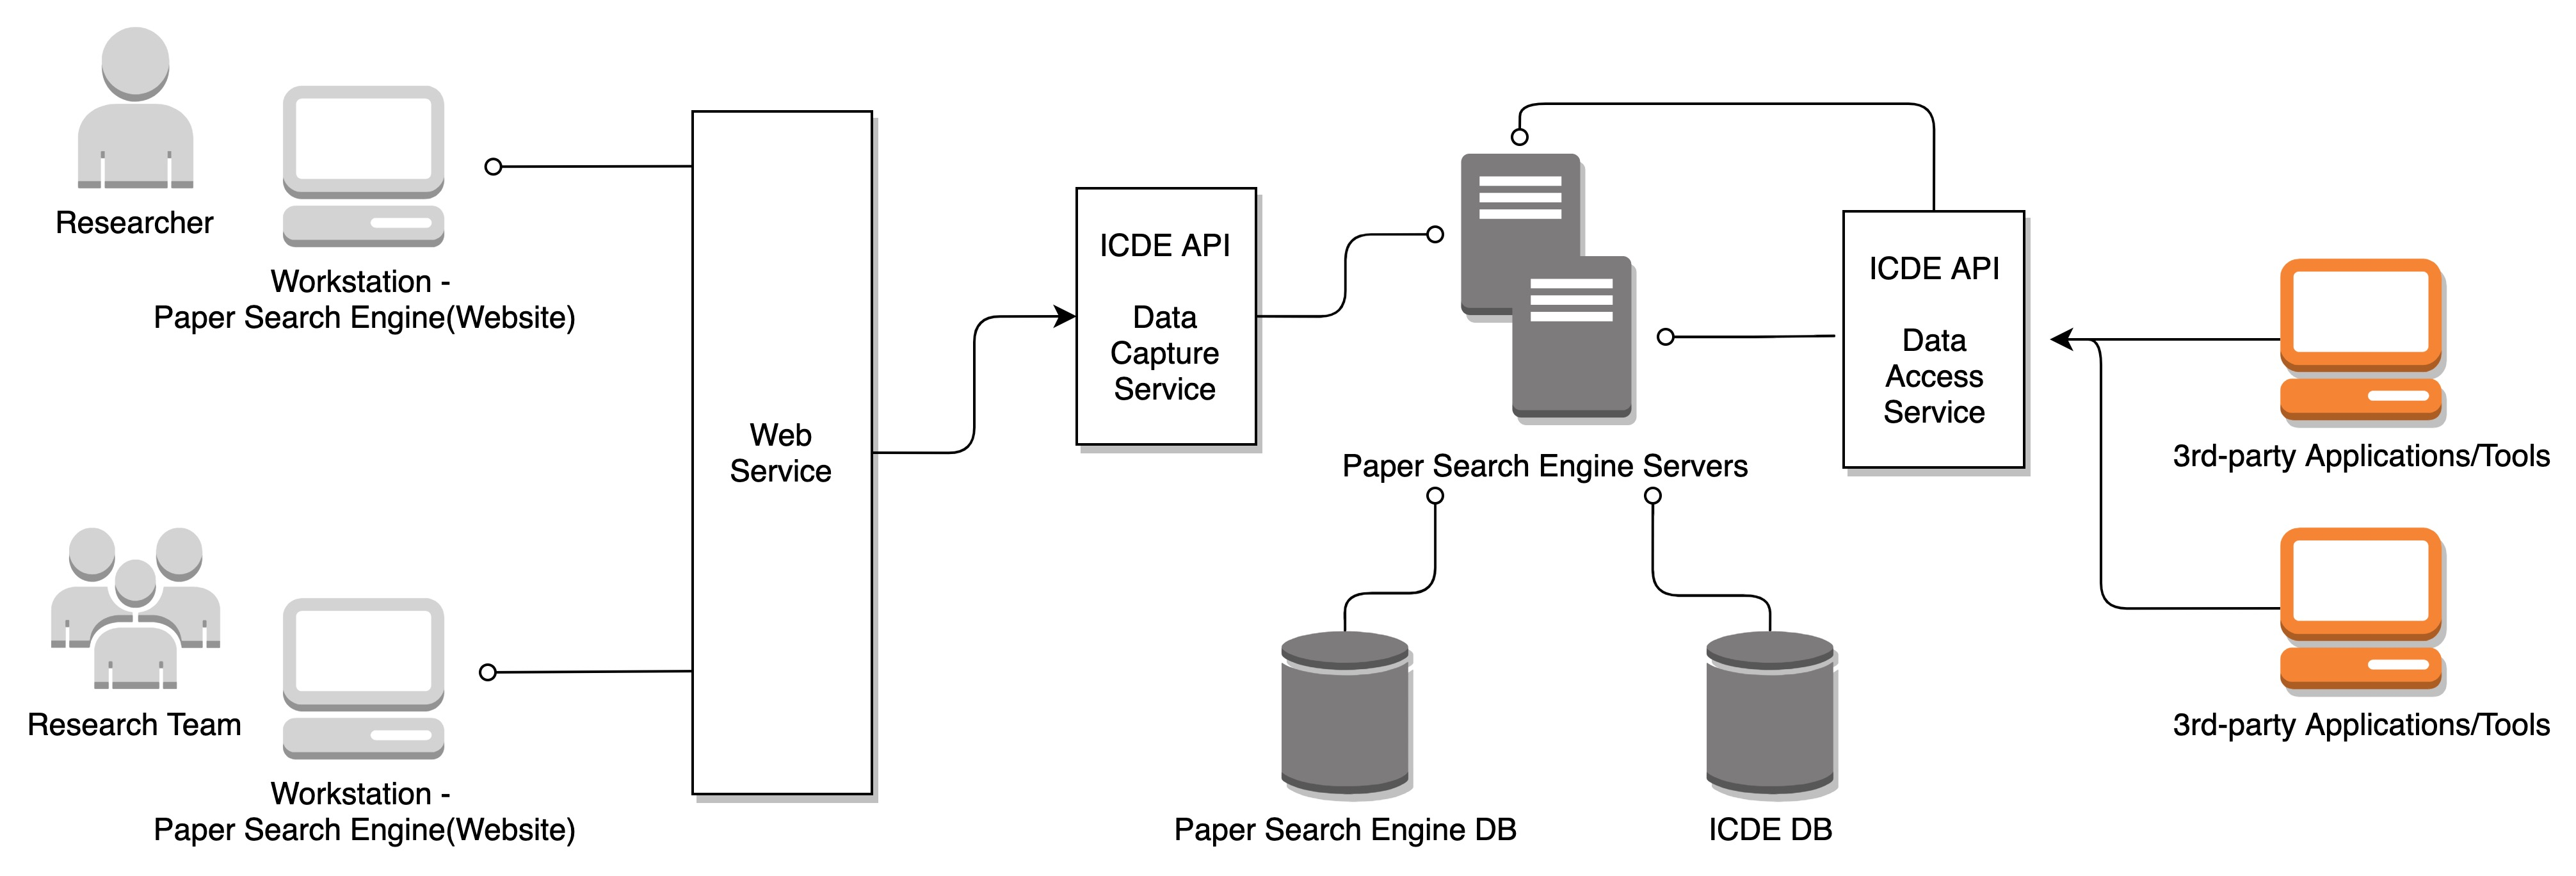
\includegraphics[scale=0.06]{sys-context.png}
	\caption{Block Diagram of the External System Arch. in Physical View}
	% 	\Description{external architectural view with block diagram}
	\label{fig:sys-context}
\end{figure}

\textbf{With the internal architecture design}, the system can be divided into three logical stacked layers
with implementing the MVC pattern\footnote{The MVC pattern introduced in the project is not exactly the same MVC pattern presented by the textbook\cite{textbook}, this will be discuss at section \ref{sec:1.3}.} at the same time.
Different layer focuses on the different logical data type as can be seen in Fig. \ref{fig:arch-dataflow}.

\begin{figure}[!ht]
	\centering
	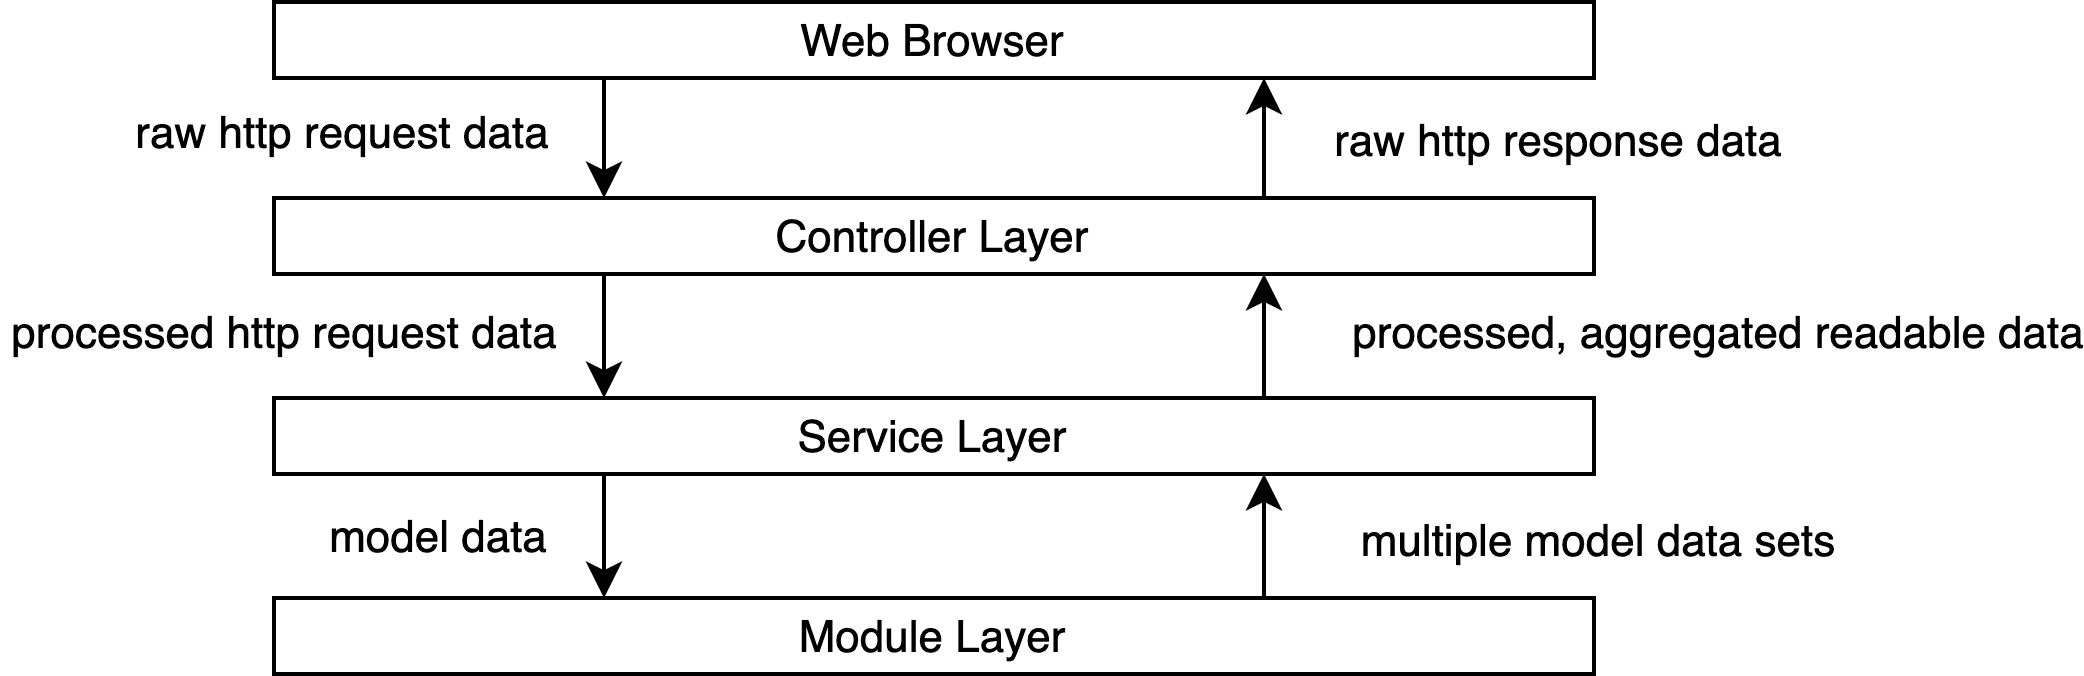
\includegraphics[width=0.48\textwidth]{arch-dataflow.png}
	\caption{The Datatype in the Layered System Architecture}
	% 	\Description{the logical view of the system architecture by layered block diagram as figure}
	\label{fig:arch-dataflow}
\end{figure}

\begin{itemize}
	\item[1] \textbf{The controller layer} contains the controllers which are responsible for receiving and responding to the HTTP requests sent from users' browsers.
		This layer is focus on the communication between the system and the browsers.
		Each controller accepts one business aspect requests and calls the corresponding service methods to retrieve the demanding data,
		and warps the date to unified standard HTTP responses which will return to the browsers.
	\item[2] \textbf{The service layer\footnote{This layer is also well known as bussiness layer/logical layer.}} contains the services which are responsible for preparing and organizing the system data.
		This layer is focus on responsing the call from controllers and calls the corresponding module methods to manipulate the data.
		Each service should abled to handle the date in bi-direction. For instance one service receives the raw data sent from the controller and do some calculation before passing the data to the presistence module.
		Or service calls methods from several persistence module and aggregates those different data sets into one set then return it to the controller.
	\item[3] \textbf{The module layer} contains two parts of the system,
		\begin{itemize}
			\item \textbf{Part one}\footnote{This part is also well known as the persistence layer.} is all about the data persistence modules which are responsible for data presistence and data query.
			      This layer part is focus on the communication between the system and the databases.
			      Each module takes the corresponding data sent from services and saves them into the databases, or queries data for the services.
			\item \textbf{Part two} is the all the other common modules or utilities that can be reused in any part of the system.
			      For instance, the common super classes or string formating handler or customized file reader etc.
		\end{itemize}

\end{itemize}

\begin{figure}[!ht]
	\centering
	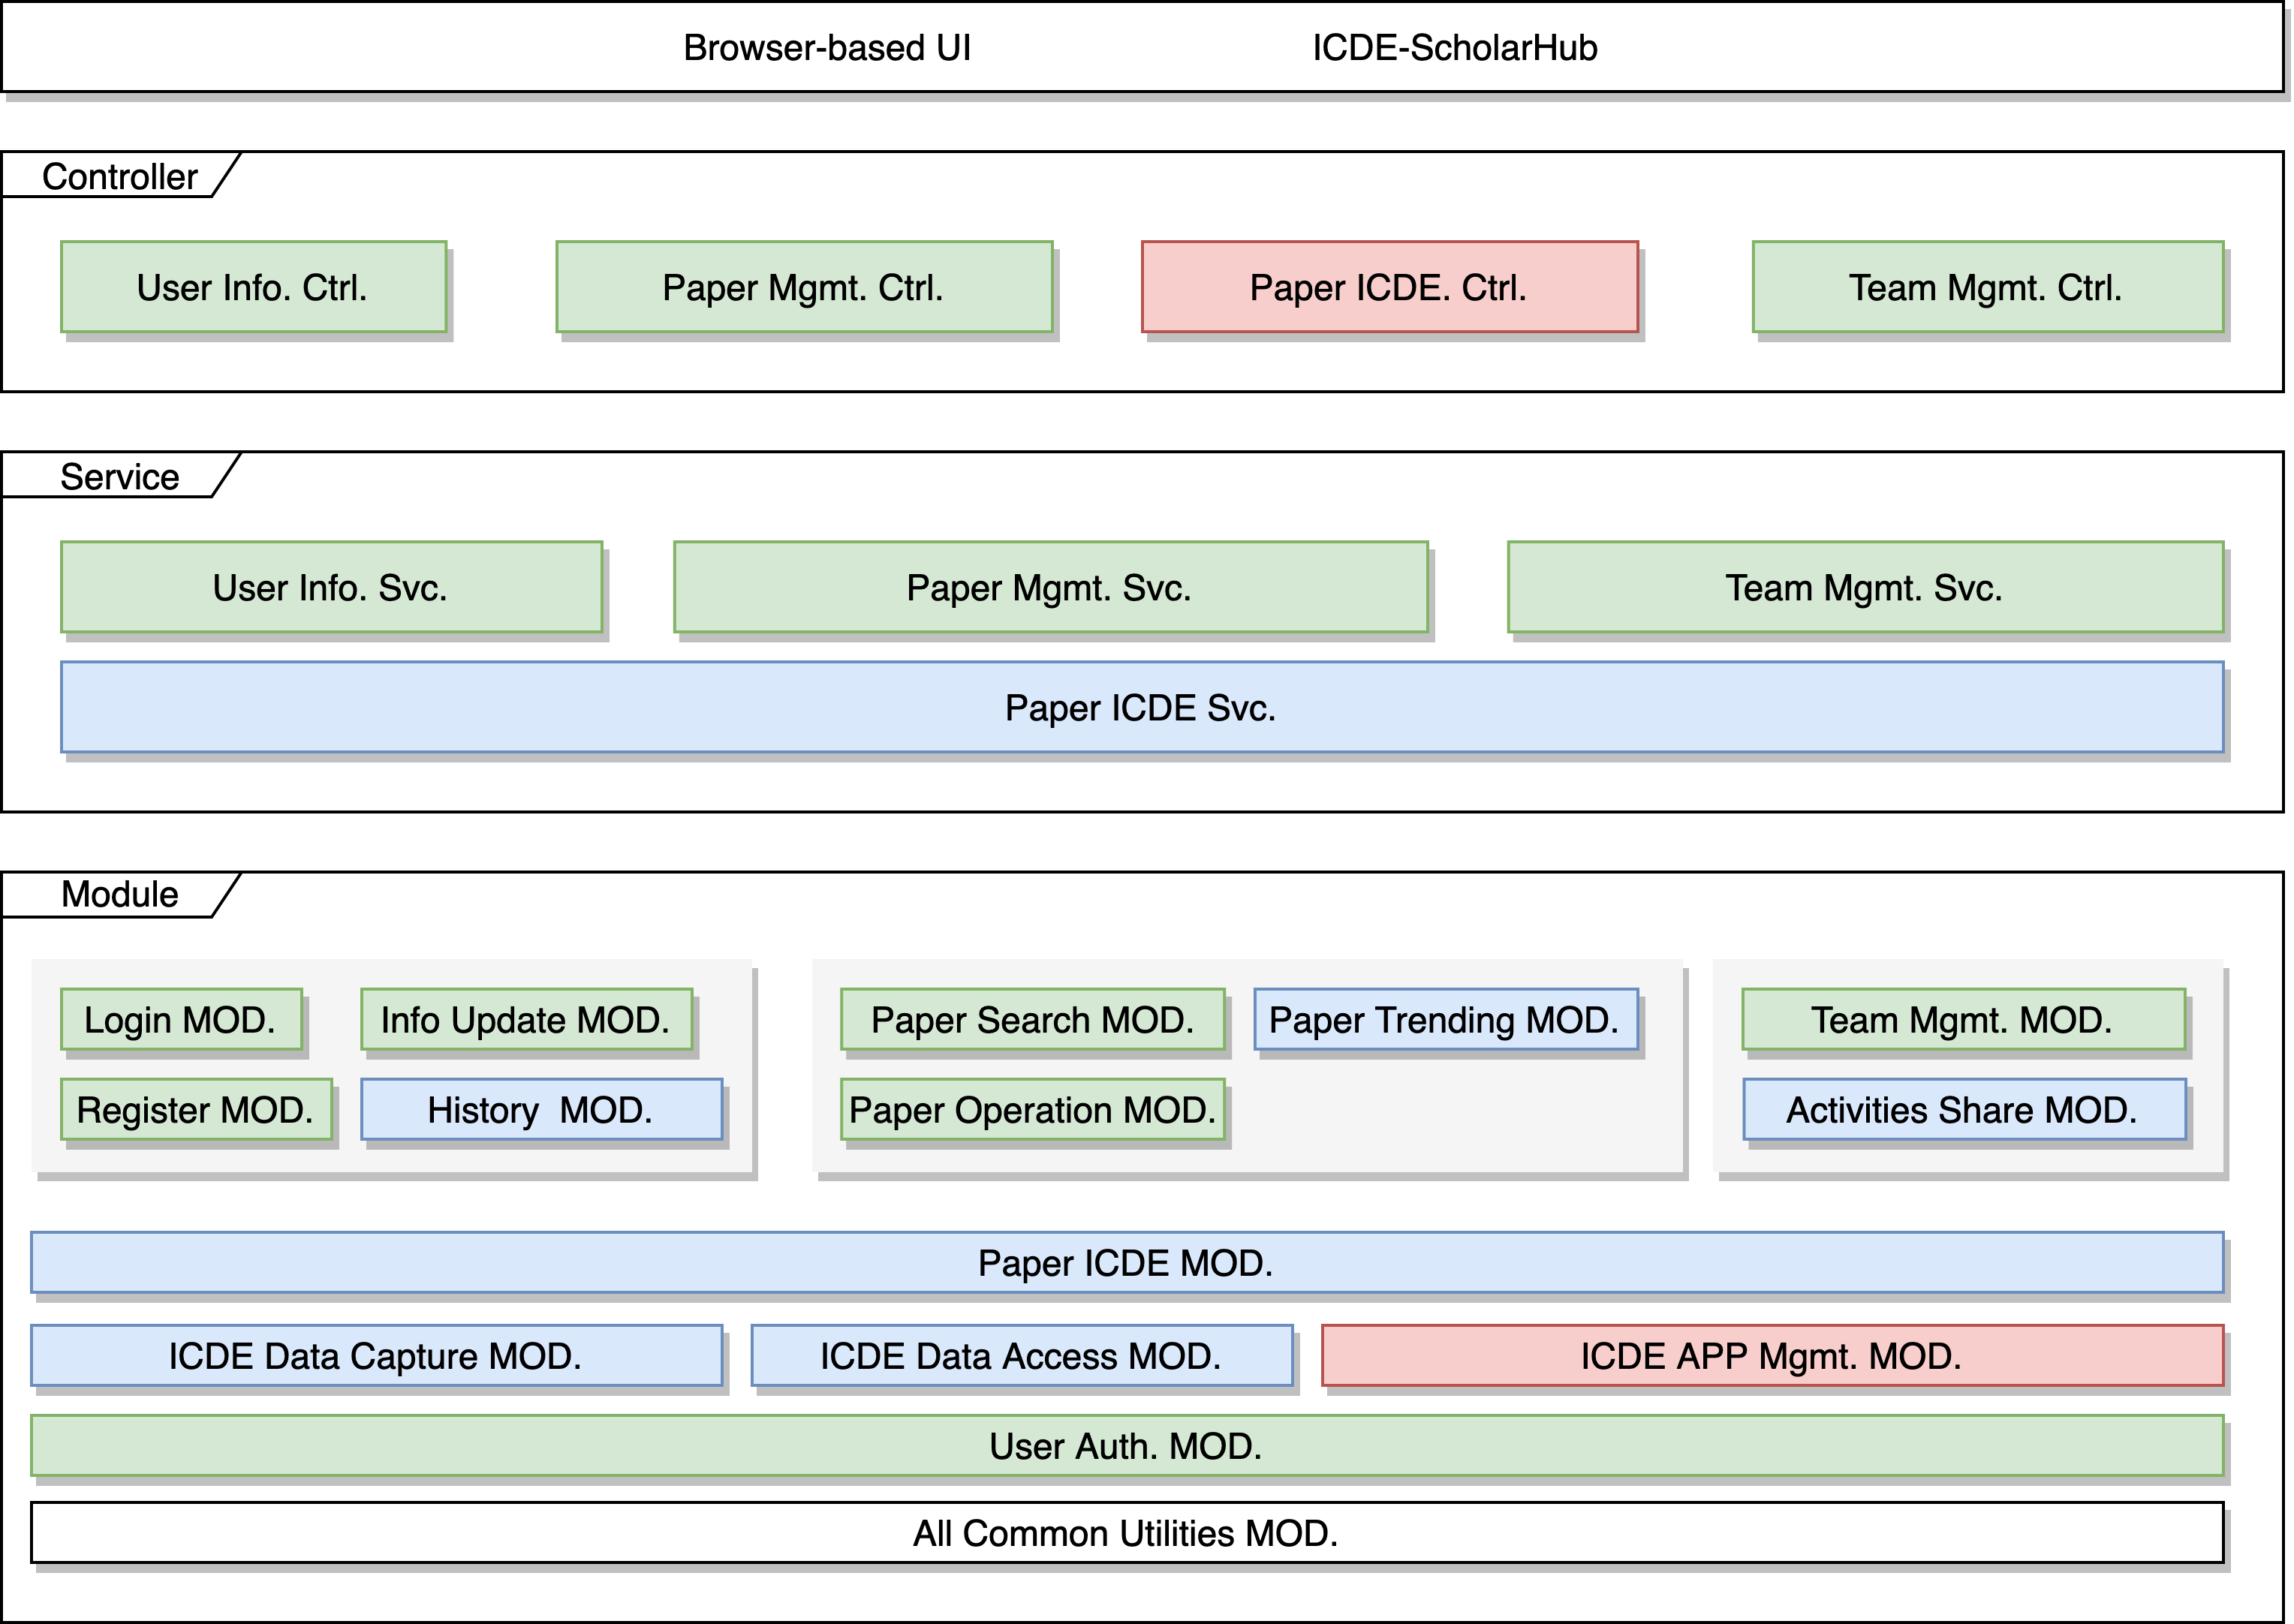
\includegraphics[scale=0.082]{sys-arch.png}
	\caption{Block Diagram of the Internal System Arch\protect\footnotemark[5]\protect\footnotemark[6]. in Logical View}
	% 	\Description{the logical view of the system architecture by layered block diagram as figure}
	\label{fig:sys-arch}
\end{figure}

\footnotetext[5]{The system architecture is different from the one which submited in the previous deliveries.}
\footnotetext[6]{Components in the green box are currently shippable, components in the blue box are on the todo list or under construction. And the components in the red box will not be implemented in the scope of the class project.}

\subsubsection{\textbf{Software Engineering Process for Designing the Architecture}}
\label{sec:1.1.2}

For how the system extrenal architecture was designed is quite simple: the project is designed to be a
web-based application, hence a trodictional B/S architecture is used to describe the
physical component of the system.

As for the internal system architecture design, the acticitiy diagram of the process is shown in Fig. \ref{fig:arch-process}.
As discussed before, each system layer was divided by what data type it handles.
Activities with the blue color are the main activities that decide how the process is perform.
And the objects with the green color are the outcome product after certain activities. After the process

\begin{figure*}[!ht]
	\centering
	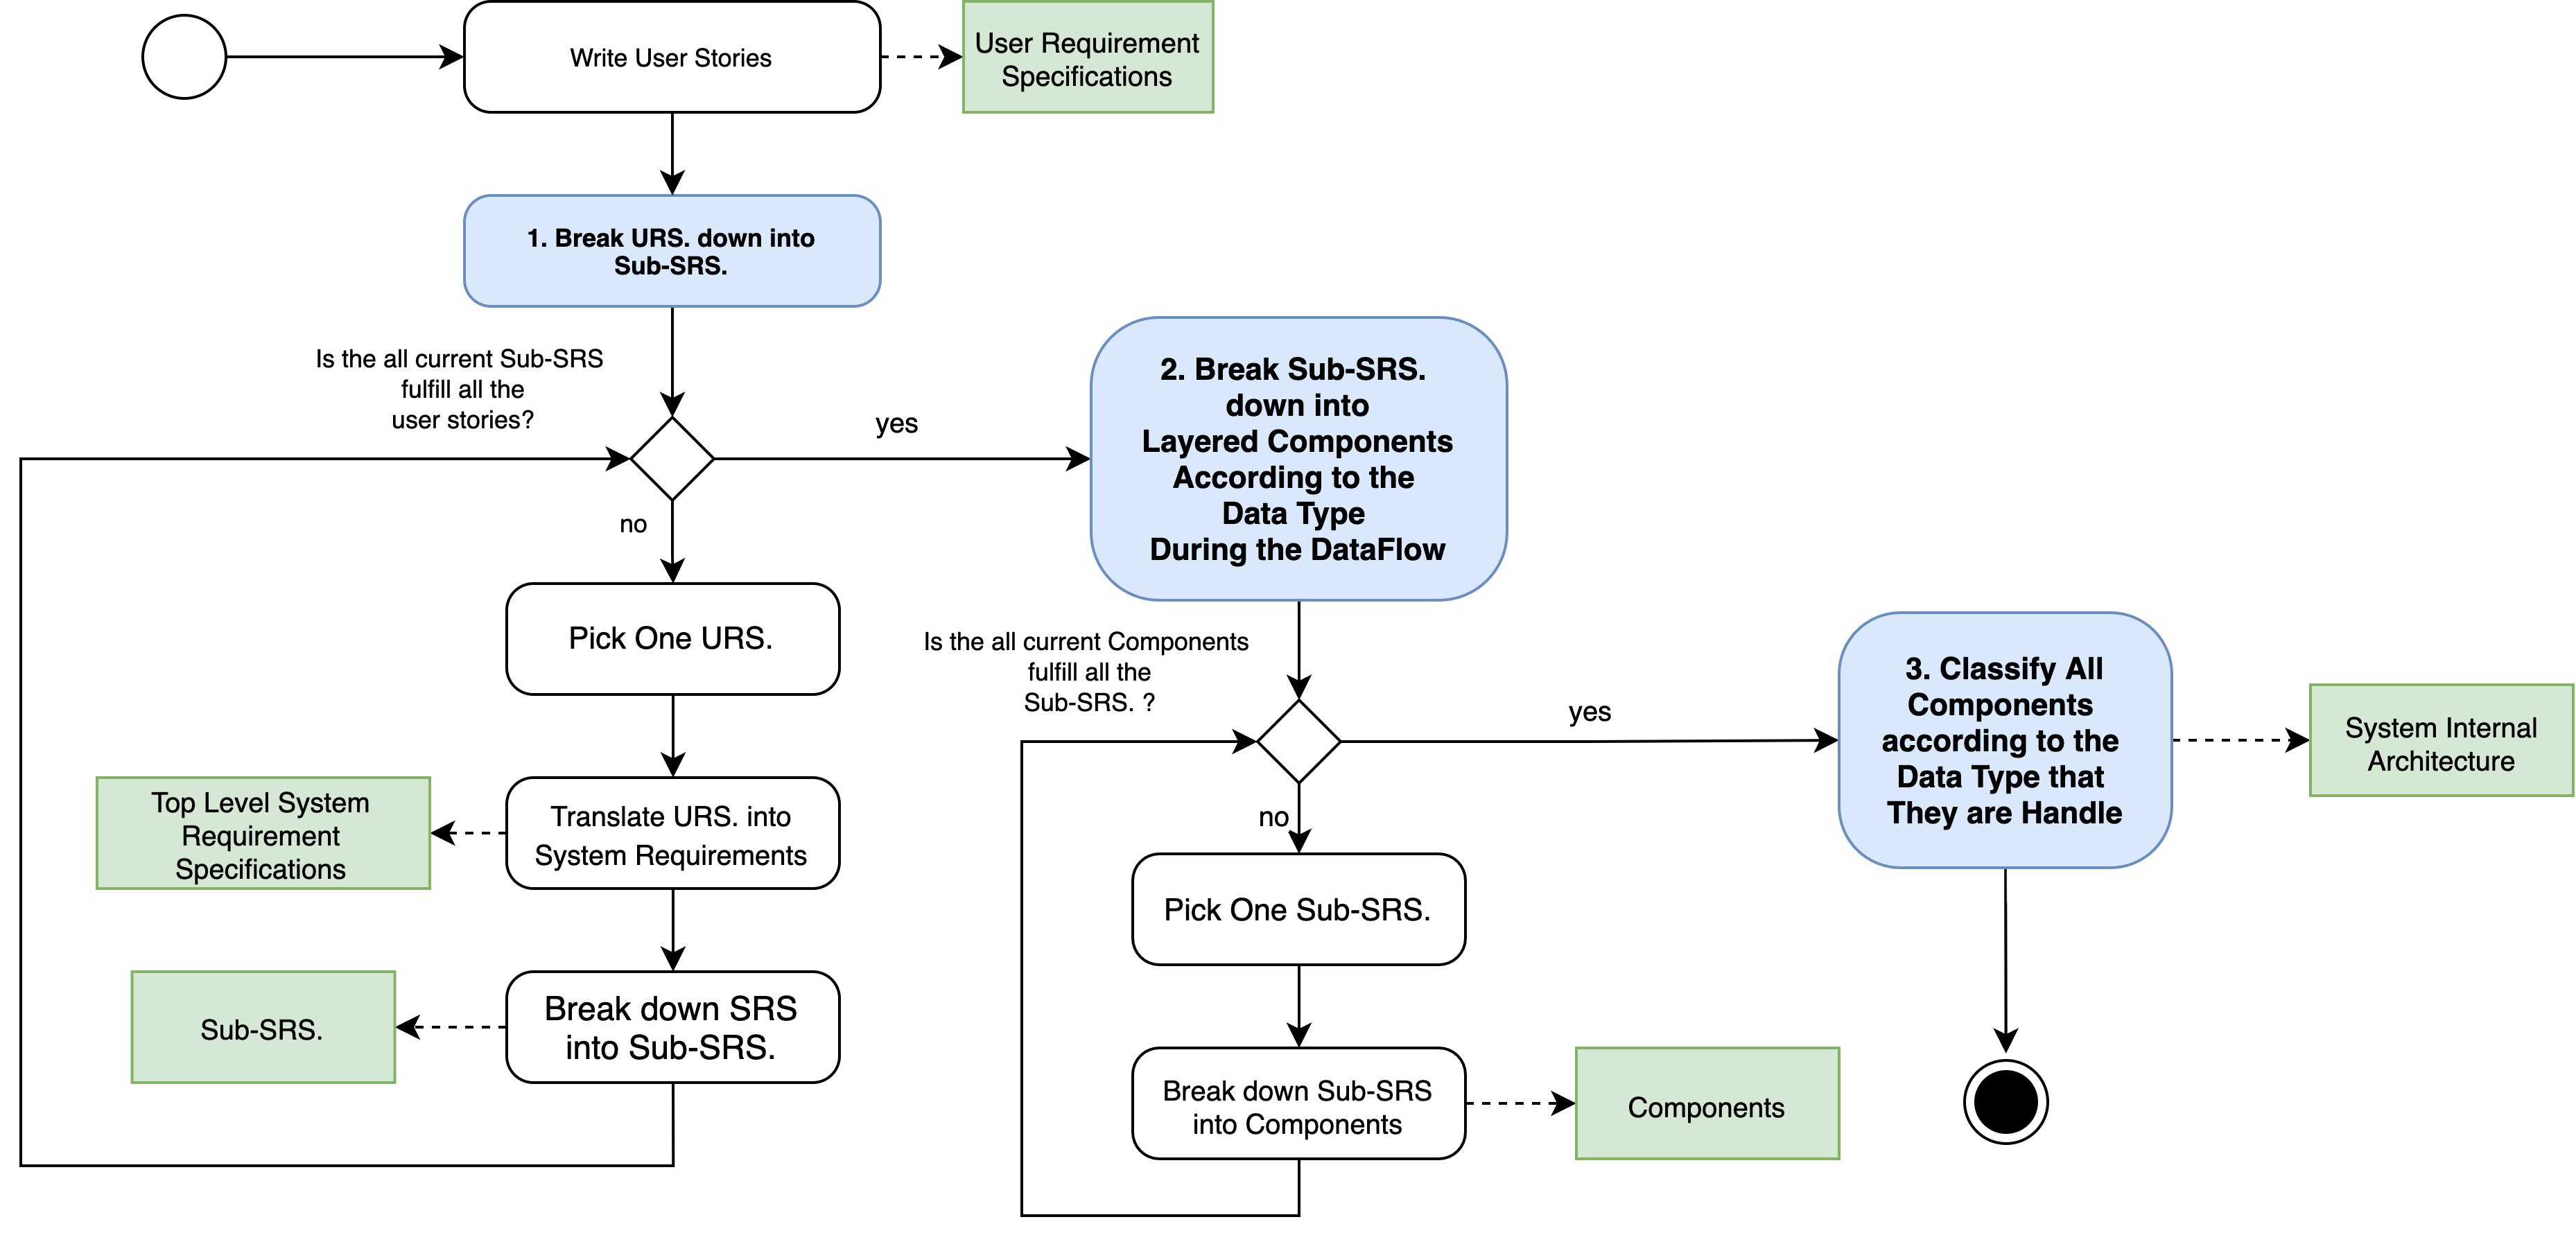
\includegraphics[width=0.9\textwidth]{arch-process.png}
	\caption{Activity Diagram of the Process for Designing the Internal System Architecture}
	\label{fig:arch-process}
\end{figure*}

\subsection{Indicate if any revision to your architectural design is necessary. If the answer is Yes, please explain what revision and the reason. }
\label{sec:1.2}

There are two reversions introduced into the system architecture during the past two sprints.
All reversions were done at the designed level before the actual code was implemented,
hence the effects of the system changing are small and smooth.

The following features were cancelled:

\begin{itemize}
	\item \textbf{Paper Upload \& Download Module:} At the initinal system requirement, the system should able to upload and download the pdf file of the paper.
	      But due to the copyright issues, the system could not maintain the pdf file database so those two features were removed.
	      Instead, the system only return an url which leads to the original paper page.
	\item \textbf{WebSocket Module:} At the initinal system requirement, team activities was designed to be updated in real-time,
	      not just polling requests by the front-end javascript so the system will maintain a websocket server for instance notification.
	      But after the latest evaluation of the user experience of the system, this real-time notification requirement is not that important.
	      So the module was removed to reduce the complexity of the system.
\end{itemize}

\subsection{Design decisions between MVC architecture pattern and layered architecture pattern.}
\label{sec:1.3}


For the internal system architectura design of this project,
\textbf{a combination of MVC architecture pattern and layered architecture pattern has been applied.}

As can be referred to\cite{mvc_versions}, there are various versions of how to interpret the Model-View-Controller over its original philosophy,
the disputable part is \textquotedblleft Can model layer be communicating with the view layer?\textquotedblright .

The version which introduced by the textbook\cite{textbook} put the answer yes on the question, which is quite disputable.
Because the mission of the model by its definition is all about managing the data,
it should never put effort into how many views are subscribing to which models and even send notification to the views.

If the answer is no, which makes sense, the MVC is actually a layered structure\cite{mvc_2,mvc_3}
since the model layer should not and should never directly communicate with the view layer.
In this report, this interpretation is marked as \textquotedblleft Layered MVC Pattern\textquotedblright
and it is what this project was following.

\subsubsection{\textbf{Adopt the Layered MVC Pattern}} how it match the internal system architecture

Fig. \ref{fig:mvc-arch} presents the project architecture from an MVC perspective view
and describes where are the scopes for Model, View, and Controller.

\begin{figure*}[!ht]
	\centering
	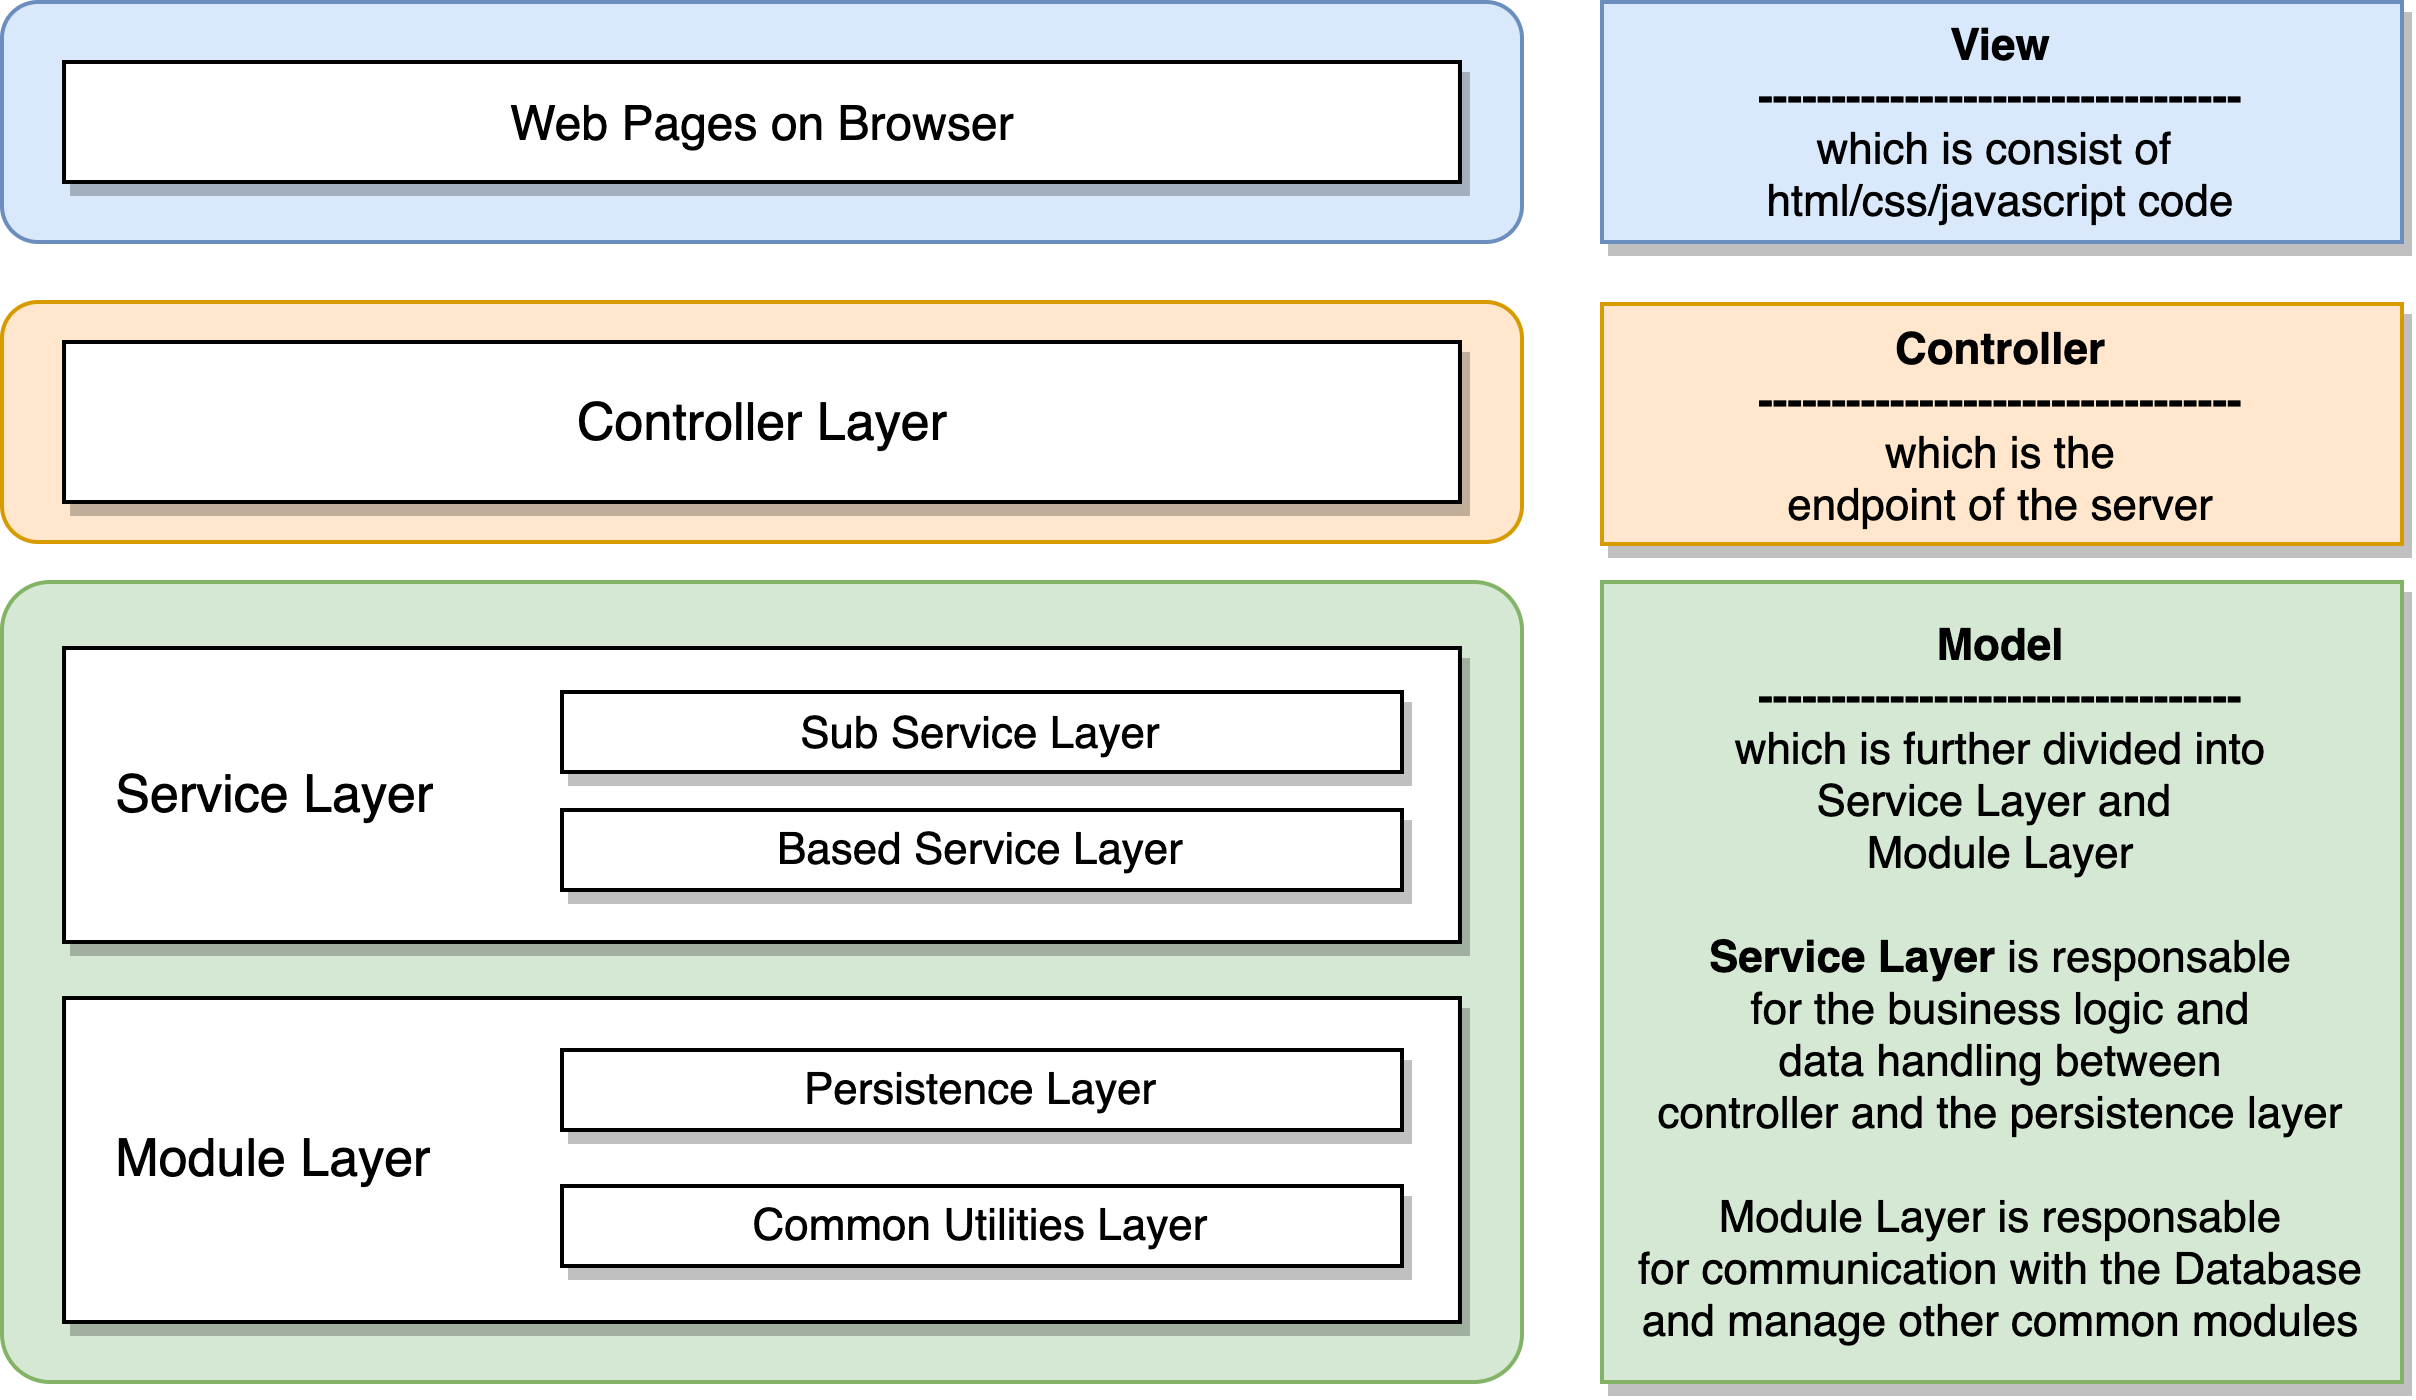
\includegraphics[width=0.7\textwidth]{mvc-arch.png}
	\caption{Matching the Layered MVC into the internal system architecture}
	\label{fig:mvc-arch}
\end{figure*}

\subsubsection{\textbf{Pros and Cons of Layered MVC}} how it affect the system and the engineering process

Advantages of MVC:
\begin{itemize}
	\item Separation of the code of front-end and back-end.
	\item Reuse of the components.
	\item Easy to maintain.
	\item Easy to test and varify the code independently.
\end{itemize}

Advantages of Layering:

\begin{itemize}
	\item Developers can focus on the layers where they were more good at.
	\item Layering the system can easily perform the data tracing during the test.
	\item Code structure is clear for reading, debuging, and for testing.
\end{itemize}

Disadvantages of both:
\begin{itemize}
	\item The structure is relatively complex for a samall project.
	      For this project, the controller layer and the service layer can be merged to one layer.
\end{itemize}

Overall, the MVC pattern and the Layer architecture pattern are share the same idea:
MVC pattern makes each part focusing on their own jobs while further layering the each part is more sensible for component separation and management.

Therefore, the project takes the advantage of this for both pattern.
A layered architecture abstracts the overall view of the system

\section{Part II}

Table \ref{tb:cc} shows the code granularity that the project has implemented so far in terms of classes/objects, packages,
libraries, frameworks and platforms.

\begin{table*}[!htb]
	\renewcommand{\arraystretch}{1.3}
	\caption{Code Granularity of the current state of the Project}
	\centering
	\begin{tabular}{p{2cm}p{1.5cm}p{2cm}p{3cm}p{1.5cm}p{3cm}l}
		\hline
		Task Name   & Tables Count & Code Level                  & Components Count & Loc & Test Cases Count & Endpoints Count \\
		\hline
		SRS 1.1     & 1            & Service                     & 1                & 70  & 4                &                 \\
		User        &              & Controller                  & 1                & 7   & 4                & 4               \\
		Information &              & Persistence\footnotemark[7] & 1                & 41  & 0                &                 \\
		Management  &              & Vue \footnotemark[8]        & 2                & 318 & 0                & 2               \\
		\hline
		SRS 1.2     & 1            & Service                     & 3                & 30  & 2                &                 \\
		Login       &              & Controller                  & 1                & 4   & 2                & 2               \\
		Logout      &              & Persistence                 & 0                & 0   & 0                &                 \\
		            &              & Vue                         & 1                & 118 & 0                & 1               \\
		\hline
		SRS 2.2     & 2            & Service                     & 1                & 176 & 5                &                 \\
		Paper       &              & Controller                  & 1                & 4   & 5                & 5               \\
		Operation   &              & Persistence                 & 1                & 31  & 0                &                 \\
		            &              & Vue                         & 1                & 531 & 0                & 1               \\
		\hline
		SRS 3.1     & 0            & Service                     & 0                & 0   & 0                &                 \\
		Paper       &              & Controller                  & 0                & 0   & 0                & 0               \\
		Search      &              & Persistence                 & 0                & 0   & 0                &                 \\
		Engine      &              & Vue                         & 1                & 531 & 0                & 2               \\
		\hline
		SRS 6.1     & 2            & Service                     & 1                & 200 & 6                &                 \\
		Team        &              & Controller                  & 1                & 11  & 0                & 6               \\
		Information &              & Persistence                 & 0                & 0   & 0                &                 \\
		Management  &              & Vue                         & 1                & 468 & 0                & 2               \\
		\hline
	\end{tabular}
	\label{tb:cc}
\end{table*}

\footnotetext[7]{The persistence layer.}
\footnotetext[8]{The view layer which use Vue Framework to implement.}

% Software metrics and granularity of components. The components’ granularity is at the level of classes/objects, packages, libraries, frameworks and platforms.

% Please make a statistical count of software metrics from all your tasks implemented so far and
% form a table given the template below.


\begin{thebibliography}{00}
	% \bibitem{mvc_1} Deacon J. Model-view-controller (mvc) architecture[J]. Online][Citado em: 10 de março de 2006.] http://www. jdl. co. uk/briefings/MVC. pdf, 2009.
	% \bibitem{layered_1} Richards, Mark. Software architecture patterns. Vol. 4. 1005 Gravenstein Highway North, Sebastopol, CA 95472: O'Reilly Media, Incorporated, 2015.
	\bibitem{textbook} Sommerville I. Software Engineering GE[M]. Pearson Australia Pty Limited, 2016.
	\bibitem{mvc_versions} Aihara D S. Study About the Relationship Between the Model-View-Controller Pattern and Usabiltity[J]. 2009.
	\bibitem{mvc_2} D. Zhang, Z. Wei and Y. Yang, "Research on Lightweight MVC Framework Based on Spring MVC and Mybatis," 2013 Sixth International Symposium on Computational Intelligence and Design, 2013, pp. 350-353, doi: 10.1109/ISCID.2013.94.
	\bibitem{mvc_3} Morse S F, Anderson C L. Introducing application design and software engineering principles in introductory cs courses: model-view-controller java application framework[J]. Journal of Computing Sciences in Colleges, 2004, 20(2): 190-201.

\end{thebibliography}


\end{document}
